\chapter{Kubernetes architecture}

\section{Etcd}
Etcd is a distributed, consistent key-value store for shared configuration and service discovery \cite{etcd}.	

\section{API server}
The Kubernetes API server validates and configures data for the API objects which include pods, services, replication controllers, and others. The API Server services REST operations and provides the frontend to the cluster shared state through which all other components interact. \cite{kubernetesdoc}

\section{Kubelet}
Another very important part of Kubernetes is Kubelet. Kubelet is an agent running on every node and it provides starting and stopping containers.

\section{Kube-proxy}
Every node in Kubernetes cluster has its own kube-proxy. This application watches the Kubernetes master node and in case of adding or deleting a service it will open or close ports (even randomly chosen) on the local node. Each connection is then forwarded to the right pod.

\begin{figure}[htb]\centering
  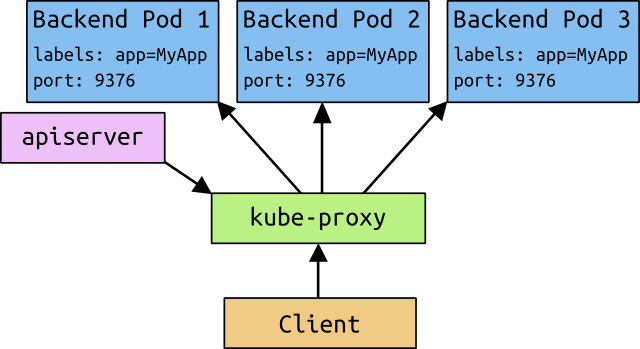
\includegraphics[width=1\textwidth]{images/services-overview.png}
  \caption
    [Service overview in Kubernetes]
    {Service overview in Kubernetes \cite{kubernetesdoc}}
  \label{fig:services-overview}
\end{figure}

\section{Controller manager}
The Kubernetes controller manager is a daemon that embeds the core control loops shipped with Kubernetes. In robotics and automation applications, a control loop is a non-terminating loop that regulates the state of the system. In Kubernetes, a controller is a control loop that watches the shared state of the cluster through the API server and makes changes in order to move the current state towards the desired state. Examples of controllers currently shipped with Kubernetes are the replication controller, endpoint controller, namespace controller, and service account controller. \cite{kubernetesdoc}

\section{Scheduler}
The Kubernetes scheduler runs as a process alongside other master components such as the API server. Its interface to the API server is to watch for pods with an empty \lstinline{PodSpec.NodeName}, and for each pod, it posts a binding indicating where the pod should be scheduled.

\begin{figure}[htb]\centering
  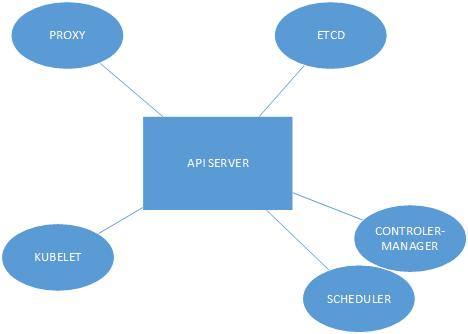
\includegraphics[width=1\textwidth]{images/kubernetes-services.png}
  \caption
    [Kubernetes services interconnection]
    {Kubernetes services interconnection \cite{tomkukral}}
  \label{fig:kubernetes-services}
\end{figure}

\section{Node}
There are two types of nodes in a cluster: the master node and the worker nodes, formerly known as minions. On the master node the API server, the scheduler and the controller manager are running together with etcd and possibly flannel. Each node runs Kubelet and optionally flannel. Using Docker for those main Kubernetes parts, the final structure of the nodes is as follows in the figure \ref{fig:kubernetes-docker-nodes}.

\begin{figure}[htb]\centering
  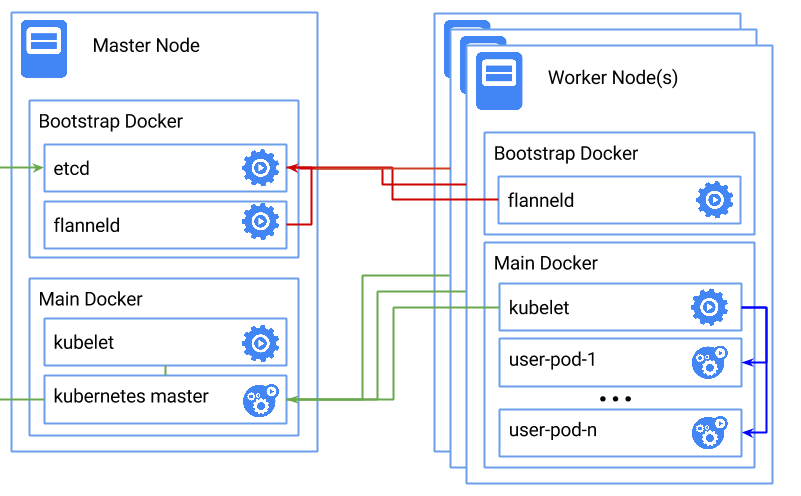
\includegraphics[width=1\textwidth]{images/k8s-docker-nodes.png}
  \caption
    [Kubernetes nodes]
    {Kubernetes nodes \cite{kubernetes-docker-multinode}}
  \label{fig:kubernetes-docker-nodes}
\end{figure}

               